En esta sección se buscan los hiperaparámetros de KNN y PCA que mejor
\emph{accuracy} score\footnote{Porcentaje de predicciones correctas} nos brinden, sin perder de vista, pero dejando en segundo

plano, el tiempo de cómputo asociado. Además respetaremos los
parámetros de tolerancia y vocabulario encontrados en las secciones
anteriores.

\subsubsection{Performance}

El primer problema con el que nos encontramos es la amplia variación
que pueden tomar los parámetros; así como los tiempos largos que
incurre el cómputo de este método.

En particular la obtención de valores singulares para lograr el
análisis de componententes principales, que ya fué mencionada en el
apartado de \emph{power method}.

Pero también la comparación de cada nuevo punto en el predict, es
altamente dependiente de la cantidad de puntos que tiene el dataset de
entrenamientos. Como se mostró en la sección de \emph{tamaño de
  muestra}, el accuracy es sensible a la cantidad de datos de
entreamiento. Por esto es que buscamos una manera de reducir la
cantidad de comparaciones que se efectúan, sin reducir la cantidad de
datos.

Para esto usamos una estructura ``arboles kd'' o ``kd-trees'' que
permiten particionar el espacio de forma binaria por dimensión y de
esta manera permiten implementaciones mucho más eficientes de KNN. Más aún, este
tipo de estructuras permite paralelismo en las queries, lo que nos permitió
pasar del orden de minutos a segundos para buscar vecinos más cercanos.

Para experimentar de manera más veloz sobre PCA también decidimos computar una
única vez los cambios de variables de la matriz sobre el mayor alfa requerido
y recortar luego componentes de esa matriz ya almacenada.

\subsubsection{Busqueda de Parámetros}

A pesar de las optimizaciones hechas, la búsqueda es intensa en tiempo
y extensa en los valores que pueden tomar los parámetros. Valores
grandes de PCA se descartan, pues uno de las características del
método es reducir la cantidad de dimensiones de los puntos
muestrales. Es decir, en nuestro caso, elegir aquellas palabras que
tienen un mayor peso en la predicción de la clasificación. Por otro
lado valores muy pequeños pueden generar pérdida de información.

Algo similar sucede con el parámetro de los vecinos, valores muy
pequeños hacen demasiado sensible al punto a ser predecido, de su
vecindad inmediata, volviendo el método sensible a las
particularidades de los datos y por lo tanto poco fiable.

Valores muy grandes de vecindad, son computacionalmente costosos y
además se pierde el sentido de vecindad que es necesario para una
clasificación exitosa. En el caso extremo, tomar como vecinos toda la
población de entrenamiento, le asignaría a cada nuevo punto el mismo
valor: aquel mayoritario en el universo.

Los valores buscados entonces, están en algún punto intermedio. Sin
embargo, este sigue siedo un intervalo bastante grande.

Con un vocabulario del orden de las 5 mil palábras y una cantidad de
datos de entrenamiento del orden de los 15 mil, tenemos un espacio
enorme para la búsqueda. Nuestra aproximación al problema, fue el de
hacer una grilla, donde se generan particiones del plano
vecinos-componentes de forma regular. Luego usar heurísticas de
búsqueda en cada una de las celdas de la misma. En particular se usó
\emph{hill climbing}\cite{aiama}\footnote{o búsqueda local, intenta en
  cada paso mejorar la solución obtenida, considerando una frontera de
  vecinos.}

Antes de seguir comentaremos rápidamente en que consistió esta metodología

\paragraph{Hillclimbing engrillado}

Por cada grilla, la heurística se mueve a pequeños intervalos
-discretos- en las cercanías de la solución obtenida, hasta llegar a
un máximo local que no puede ser mejorado.  La figura
\ref{fig:hill-choreado} muestra la idea de \emph{hillclimbing} en una
búsqueda de una dimensión.
 
La definición de estos pequeños intervalos, está relacionada con el
tamaño de cada celda por un lado y por otro de la cantidad de
iteraciones que hará la búsqueda local hasta alcanzar un máximo. 

\begin{figure}[ht]
  \begin{subfigure}{.5\textwidth}
  \begin{center}
    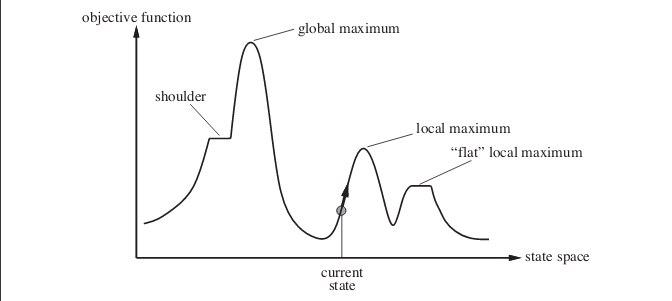
\includegraphics[width=1.0\textwidth]{./img/hillclimbing-choreado.png}
  \end{center}
  \caption{Búsqueda local o hillclimbing en un caso hipotético sobre
    una dimensión. La heurística permite reducir el espacio de
    búsqueda, pero puede caer en extremos locales sub óptimos.}
  \label{fig:hill-choreado}
  \end{subfigure}
  \begin{subfigure}{.5\textwidth}
    \begin{center}
      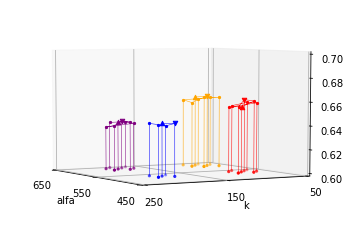
\includegraphics[width=1.0\textwidth]{./img/hillclimbing-1.png}
    \end{center}
    \caption{Hill climbing engrillado. Perspectiva 1.}
    \label{fig:hill-1}
  \end{subfigure}
  \begin{subfigure}{.5\textwidth}
    \begin{center}
      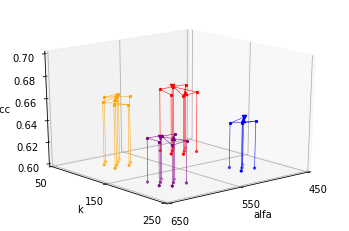
\includegraphics[width=1.0\textwidth]{./img/hillclimbing-2.png}
    \end{center}
    \caption{Hill climbing engrillado. Perspectiva 2.}
    \label{fig:hill-2}
  \end{subfigure}
  \begin{subfigure}{0.5\textwidth}
    \begin{center}
      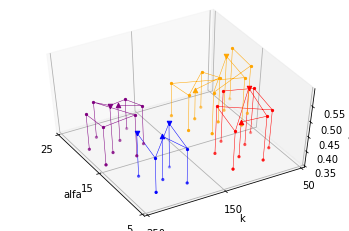
\includegraphics[width=1.0\textwidth]{./img/hillclimbing-3.png}
    \end{center}
    \caption{Hill climbing engrillado. Perspectiva 3.}
    \label{fig:hill-3}
  \end{subfigure}
  \caption{De (b) a (d) se muestran distintas perspectivas de la
    partición del espacio en 4 celdas de 100x10 (k x $\alpha$). En
    distintos colores cada búsqueda local. Los triángulos que apuntan
    hacía arriba indican de donde comienza la búsqueda. Los que
    apuntan hacia abajo, el máximo valor encontrado. Estos últimos
    suelen no ser el último valor de la búsqueda, porque para saber
    que es un máximo el algoritmo tiene que ver todos los
    vecinos. Esto explica que la linea que une el orden de visita, no
    sea una curva ascendente monotónica si no un zig-zag de ascenso y
    descenso.}
\end{figure}

Esto último se debe a que los intervalos son discretos, entonces
cuanto más grandes son, menos soluciones estamos considerando y es más
corto el camino hacía un máximo que no se pueda mejorar (lo que no
significa que esa un máximo real).  En las figuras \ref{fig:hill-1}
\ref{fig:hill-2} \ref{fig:hill-3} mostramos como se generan los
heatmaps, tomando el mayor de los valores en cada celda.

Esta metodología nos permite reducir mucho el espacio de búsqueda. Por
poner un ejemplo de una grilla de 100x100, donde se efectúa una
búsqueda local considerando 200 elementos, pagamos un costo
$\frac{200}{100^2} = 0,002$ menor al de explorar toda la grilla y es
sensiblemente mejor que simplemente tomar un punto arbitrario de la
misma.

\paragraph{Busqueda iterativa engrillada de escaladores:}

Para la definición de los parámetros de la búsqueda local, tuvimos en
cuenta las consideraciones anteriores y generamos varias
grillas. Primero una de gran tamaño (componentes principales entre 100
y 1000 con cantidad de vecinos de hasta 2000, guiandonos por el pico
de la curva de la experimentación de kNN sin PCA) que nos permitiera
analizar el relieve general y buscar mesetas sobre las cuales hacer
distintos ``zooms'' con mayor granularidad enfocados en regiones
específicas de interés, luego una más pequeña con valores chicos de
alfa y k cercanos a una meseta en particular inspirados por las
grillas anteriores.

En el panorama mascroscópico de la figura \ref{fig:pca-big} se puede
notar una característica positiva respecto de nuestro método de
experimentación: la imagen de la función a maximizar es muy suave, lo
que es favorable para el hillclimbing frente a superficies más
``cerruchadas'' y que nos permite tener más confianza en los máximos
locales obtenidos como posibles máximos globales de cada celda (lo que
significa necesitar menos iteraciones de ``zooms'' para análisis
exhaustivos). Otra particularidad interesante es que la función se
comporta muy parecido al caso que vimos optimizando sin PCA: alcanza
buenos valores con pocos ($<150$) vecinos, luego empeora y cerca de
los 2000 vecinos se vuelve a comportar de manera precisa. Si bien
analizaremos con más detalle ambas mesetas, asumiendo que la suavidad
de la función nos indica que los máximos encontrados son esos y que
ninguna supera a la otra, decidimos descartar aquellas combinaciones
con valores grandes de k o alfa (en el caso de que no haya picos
dominantes en tal región) por cuestiones de tiempo de cómputos dado
que, sobre esa misma frontera de nuestra región total, se vuelven muy
poco prácticas tales latencias.

En el zoom de la región de parámetros grandes visto en la figura
\ref{fig:pca-z1} se valida nuestra suposición de que la suavidad de la
imagen de la función objetivo implicaría buena representatividad de
los máximos locales hallados con granularidades más altas: muy pocas
celdas superan el $0.66$ de accuracy score correspondiente a las
respectivas zonas del muestreo panorámico anterior. Si la imagen de la
función diera saltos crecerían nuestras chances de encontrar picos
puntuales en análisis más microscópicos. Como dijimos, esto nos
permite descartar la región en favor de valores más pequeños con menos
latencia asociada y misma precisión.

En la figura \ref{fig:pca-z2} el zoom de la región de parámetros
pequeños nos muestra que los valores cercanos al 0.68 de la función
objetivo están pegados a la frontera contraria del zoom anterior: son
valores mucho más chicos de lo que esperábamos dado nuestro rango
original. Si bien esto significaría buenos resultados con poco costo
de performance, como ya analizamos, valores pequeños de estos
parámetros podrían significar menor tolerancia a ruidos muestrales
(por ejemplo mayor variación entre predicciones de distintos
datasets)\footnote{Situación que pudimos comprobar al pasar del set de
  testing de 6000 casos de imdb\_small al set de 100 de test\_sample
  de la cátedra, donde el comportamiendo se volvía más errático
  seguramente por cuestiones de tamaño muestral.}.

Habiendo visto que valores particularmente grandes de nuestros
parámetros no mejoraban la función objetivo tanto como esperábamos y
que el rango macroscópico original que planteamos no parecía del todo
concluso decidimos extender el espacio de búsqueda buscando valores
aún más pequeños con los resultados vistos en la figura
\ref{fig:pca-small} donde la franja 40-52 para k y 150-350 para alfa
supera los demás resultados vistos anteriormente.

De este modo no pudimos superar en una primera iteración de grillas y
parámetros iniciales los resultados de kNN sin PCA agregando tal
método. Esto no significa que tras ajustes en otros parámetros que
afectan al método (como aquellos de la vectorización o el dataset de
entrenamiento mismo) no podamos reiterar las experimentaciones
mejorando los resultados y progresando sobre estos, además de que la
cualidad de seleccionar componentes con mucha cohesión interna
respecto de la vectorización original es muy útil para eliminar ruidos
muestrales significando mayor estabilidad a cambios en datasets de
entrenamiento y testeo que sin PCA.

Cabe destacar que según se acostumbra en procesamiento de
lenguaje\cite{LP} natural\footnote{In general (Gale and Church, 1990)
  suggest that the vocabulary size (the number of types) grows with at
  least the square root of the number of tokens (i.e.
  $V > O(\sqrt{N})$.} la cantidad de vocabulario se suele tomar como
función creciente de la raiz cuadrada de los tokens\footnote{Tomamos
  vocabulario, como types. Los tokens son todas las entidades
  identificables en un corpus (una colección de textos) Puede incluir
  hasta signos de puntación. Los types/tipos, son las palabras
  utiles.}, y que según nuestros datos, la raiz es un valor que ronda
los 300\footnote{El valor no es exacto porque depende de como se
  consideren los tokens}; bien dentro de la franja de componentes
principales, que mencionamos antes.

\begin{figure}[h]
  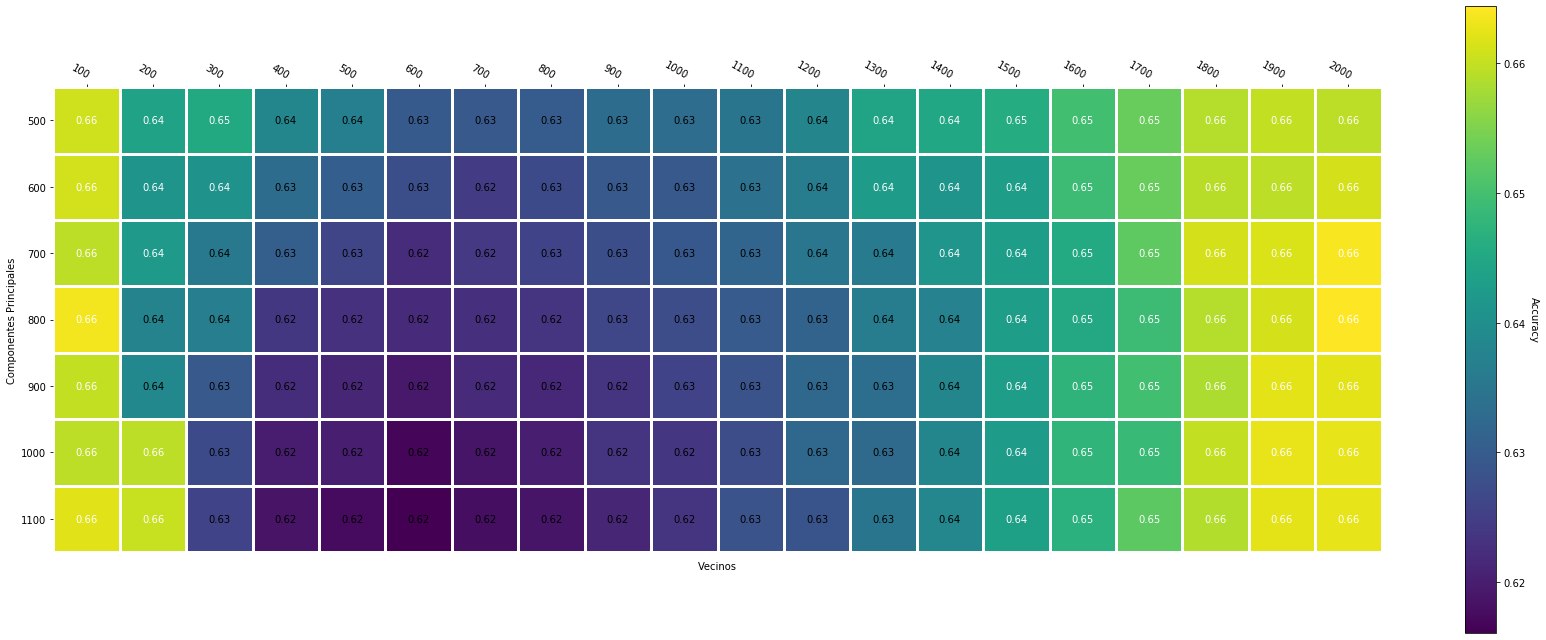
\includegraphics[width=1.05\textwidth]{./img/pca_big_grid.png}
  \centering
  \caption{Resultado de la busqueda local sobre cada región
    \textbf{grande} de k100x$\alpha$100. En cada una de las celdas se corrió una búsqueda local con ``steps" de 10 unidades sobre ambos parámetros comenzando en el valor mostrado en los ejes hasta alcanzar un
    máximo local. Se muestran sobre el color, el accuracy logrado por el máximo local.}
  \label{fig:pca-big}
\end{figure}


\begin{figure}[h]
    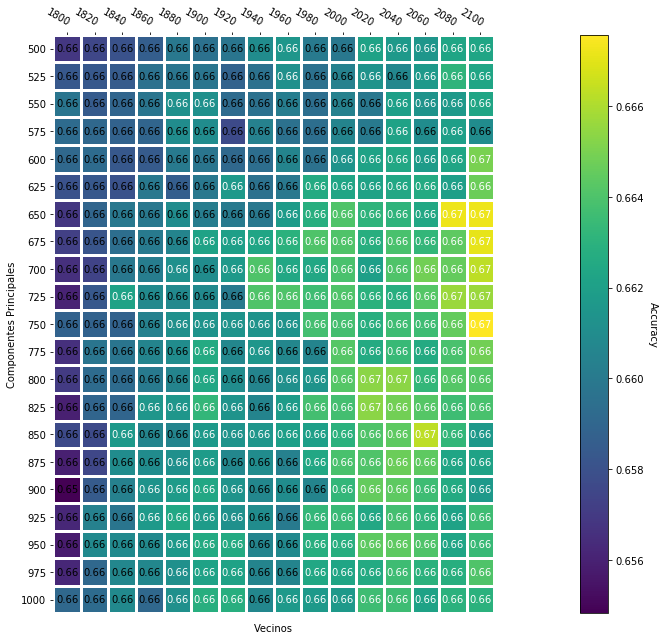
\includegraphics[width=0.7\textwidth]{./img/pca_zoom1_grid.png}
    \centering
    \caption{Resultado de la busqueda local sobre cada región de k20x$\alpha$25 del \textbf{zoom sobre la meseta de valores altos de cantidad de vecinos}. En cada una de las celdas se corrió
    una búsqueda local con ``steps" de 5 unidades para ambos parámetros comenzando en el valor mostrado en los ejes
    hasta alcanzar un \textbf{máximo local}. Se muestran sobre el color, el accuracy logrado
    por el máximo local.}
    \label{fig:pca-z1}
\end{figure}

\begin{figure}[h]
    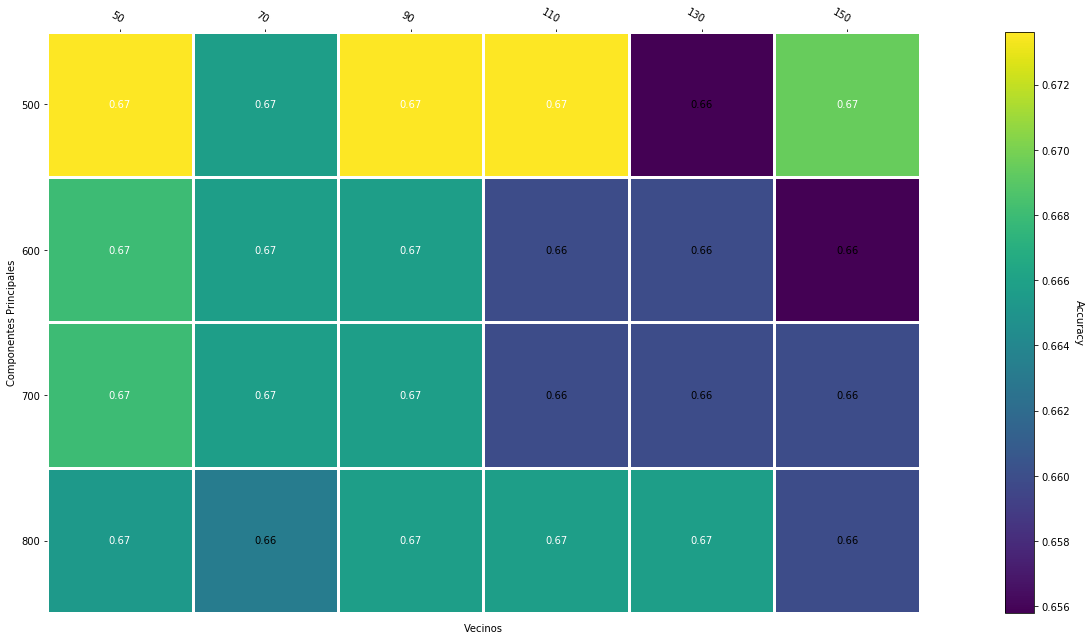
\includegraphics[width=0.8\textwidth]{./img/pca_zoom2_grid.png}
    \centering
    \caption{Resultado de la busqueda local sobre cada región de k20x$\alpha$100 del \textbf{zoom sobre la meseta de valores chicos de cantidad de vecinos} . En cada una de las celdas, se corrió
    una búsqueda local con ``steps" de 10 para la cantidad de vecinos y 50 para la cantidad de componentes principales comenzando en el valor mostrado en los ejes
    hasta alcanzar un \textbf{máximo local}. Se muestran sobre el color, el accuracy logrado
    por el máximo local.}
    \label{fig:pca-z2}
\end{figure}

\begin{figure}[h]
  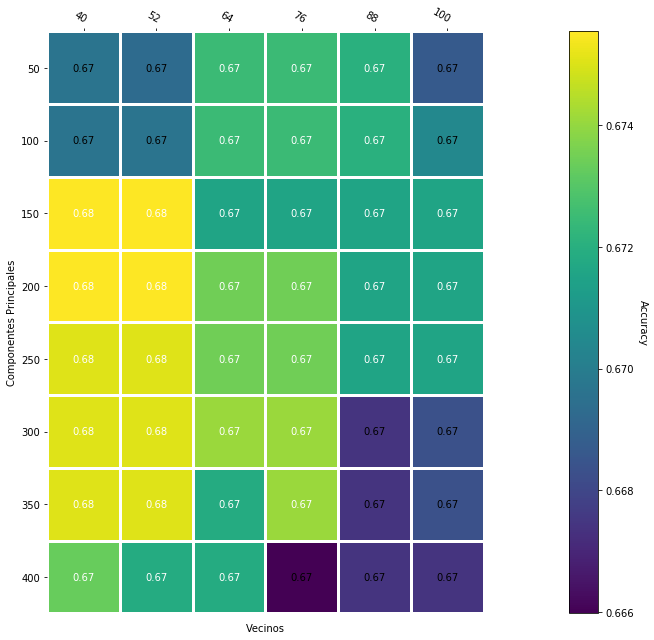
\includegraphics[width=0.5\textwidth]{./img/pca_big_ext.png}
  \centering
  \caption{Resultado de la busqueda local sobre cada región
    \textbf{chica} de k12x$\alpha$50. En cada una de las celdas, se corrió
    una búsqueda local con ``steps" de 6 para la cantidad de vecinos y 25 para la cantidad de componentes principales comenzando en el valor mostrado en los ejes
    hasta alcanzar un \textbf{máximo local}. Se muestran sobre el color, el accuracy logrado
    por el máximo local.}
    \label{fig:pca-small}
\end{figure}
